\documentclass[aspectratio=169]{beamer}

\usetheme{CambridgeUS}
\usecolortheme{default}
\useinnertheme{default}
\useoutertheme{default}

\setbeamertemplate{navigation symbols}{}
\setbeamertemplate{footline}[frame number]
\setbeamertemplate{itemize item}{\textbullet}
\setbeamertemplate{itemize subitem}{--}

\setbeamercolor{title}{fg=black}
\setbeamercolor{frametitle}{fg=black}
\setbeamercolor{structure}{fg=black}
\setbeamercolor{normal text}{fg=black}
\setbeamercolor{alerted text}{fg=black!80}
\setbeamercolor{block title}{fg=black,bg=black!8}
\setbeamercolor{block body}{fg=black,bg=black!3}
\setbeamercolor{block title alerted}{fg=white,bg=black!70}
\setbeamercolor{block body alerted}{fg=black,bg=black!5}
\setbeamercolor{block title example}{fg=white,bg=black!50}
\setbeamercolor{block body example}{fg=black,bg=black!5}

\setbeamerfont{title}{size=\Large,series=\bfseries}
\setbeamerfont{frametitle}{size=\large,series=\bfseries}
\setbeamerfont{block title}{series=\bfseries}

\usepackage{booktabs}
\usepackage{amsmath}
\usepackage{amssymb}
\usepackage{graphicx}
\usepackage{threeparttable}

\title{Bayesian Market Concentration for Multi-Sector Firms}
%\subtitle{Evidence from U.S.\ Public Firms, 2017--2025}
\author{Zifan Huang}
\date{April 29, 2026}
\institute{Chicago Booth}

\begin{document}

\begin{frame}[plain]
  \titlepage
\end{frame}

% ================================================
% MOTIVATION
% ================================================

\begin{frame}{The HHI Has a Measurement Problem}

  \textbf{Standard HHI/CR4 treats firm-industry assignment as known.}

  \vspace{1em}

  \textbf{Amazon North America (FY2024, \$386B):}
  \begin{itemize}
    \item Groceries (Whole Foods + Fresh)
    \item General merchandise
    \item Consumer electronics
    \item Digital content + Prime
  \end{itemize}

  \vspace{1em}

  All of this gets one NAICS code. Which market is Amazon in?

  \vfill
  \textbf{When the code changes, HHI jumps---not because competition changed.}

\end{frame}

\begin{frame}{What We Know (and Don't)}

  \textbf{Rising U.S.\ concentration is well-documented:}
  \begin{itemize}
    \item Grullon, Larkin, Michaely (2019): 75\% of industries more concentrated, 1997--2014
    \item Autor et al.\ (2020): superstar firms capture rising revenue share
  \end{itemize}

  \vspace{1em}

  \textbf{But every study treats the firm-industry map as fixed.}

  \vspace{1em}

  \begin{block}{Question}
    How much of measured concentration is real consolidation versus an artifact of arbitrary NAICS assignment?
  \end{block}

\end{frame}

% ================================================
% THIS PAPER
% ================================================

\begin{frame}{This Paper}

  \begin{itemize}
    \item Treat firm-industry allocation as a latent variable, identify it from Compustat NAICS co-occurrence, and propagate posterior uncertainty into concentration measures.
  \end{itemize}

  \vspace{1.5em}

  \textbf{Main findings:}
  \begin{enumerate}
    \item Aggregate HHI rose $\approx$330 points (18\%) from 2022 to 2025
    \item On average, standard benchmark \textbf{overstates} concentration but \textbf{understates} growth over time
    \item Benchmark 2025 HHI lies in \textbf{right tail} of Bayesian posterior
  \end{enumerate}

\end{frame}

% ================================================
% DATA
% ================================================

\begin{frame}{Data: WRDS API Compustat Segment Panel}

  \textbf{Source:} Compustat \texttt{wrds\_segmerged}, 2017--2025

  \vspace{0.8em}

  \begin{columns}[T]
    \begin{column}{0.48\textwidth}
      \textbf{Sales panel}
      \begin{itemize}
        \item 19{,}302 segment-year obs
        \item 2{,}932 unique firms
        \item 241 current S\&P 500 members
        \item S\&P 500 = 60\% of total sales
        \item S\&P 500 median: \$6.8B/segment
      \end{itemize}
    \end{column}
    \begin{column}{0.48\textwidth}
      \textbf{NAICS count panel}
      \begin{itemize}
        \item 41{,}844 segment-industry rows
        \item 862 unique NAICS codes
        \item Mean count per row: 2.91
        \item Max: 12 NAICS codes/segment
        \item Counts $\to$ Dirichlet prior $\alpha_0$
      \end{itemize}
    \end{column}
  \end{columns}

  \vfill
  \small\textit{Stable coverage 2019--2022 ($\approx$2{,}200 firms/yr). Partial-year attrition in 2024--2025.}

\end{frame}

% ================================================
% MODEL
% ================================================

\begin{frame}{Model: Bayesian Dirichlet Allocation}

  \small\textit{Indices: $f$ = firm, $s$ = segment $\in f$, $k$ = industry, $t$ = year, $r$ = draw}

  \vspace{0.4em}

  \textbf{Prior} Sales-weighted pseudo-counts (summed over pre-period $\mathcal{T}_0 = 2017$--$2021$):
  \[
    \alpha_{fs,k}^{(0)} = \sum_{t\in\mathcal{T}_0}
      \underbrace{\frac{c_{fs,k,t}}{C_{k,t}} \cdot S_{k,t}}_{w_{fs,k,t}:\;\text{segment's share of industry }k\text{'s count} \times \text{industry sales}} + \;\varepsilon
  \]

  \textbf{Closed-form posterior} for segment $(f,s)$ in year $t$:
  \[
    \pi_{fs,\cdot,t}\mid\text{data} \sim \mathrm{Dirichlet}\!\bigl(\alpha_{fs,\cdot}^{(0)} + w_{fs,\cdot,t}\bigr)
  \]

  \textbf{Posterior draws} ($R=500$) are taken from this known distribution only to propagate uncertainty into HHI and CR4:
  \[
    \pi_{fs,\cdot}^{(r)} \sim \mathrm{Dirichlet}\!\bigl(\alpha_{fs,\cdot}^{(0)} + w_{fs,\cdot,t}\bigr),
    \quad \pi_{fs,k}^{(r)} = \text{drawn share of }(f,s)\text{'s revenue in }k
  \]

  \textbf{Firm imputed revenue} in industry $k$, year $t$, draw $r$:
  \[
    \tilde{r}_{f,k,t}^{(r)} = \sum_{s \,\in\, f} \pi_{fs,k}^{(r)} \cdot r_{fs,t}
    \;\Rightarrow\; \text{market shares} \to \text{HHI, CR4.}
  \]

  \vfill
  \textbf{Benchmark} (no draws): fixed $\hat\pi_{fs,k,t} = c_{fs,k,t}/\!\sum_{k'} c_{fs,k',t}$ (raw count, normalized in year $t$)\\
  $\Rightarrow$ single firm-level revenue $\hat{r}_{f,k,t} = \sum_{s\,\in\,f} \hat\pi_{fs,k,t}\cdot r_{fs,t}$.

\end{frame}

% ================================================
% MAIN RESULT
% ================================================

\begin{frame}{Aggregate HHI Rose 330 Points, 2022--2025}

  \begin{center}
    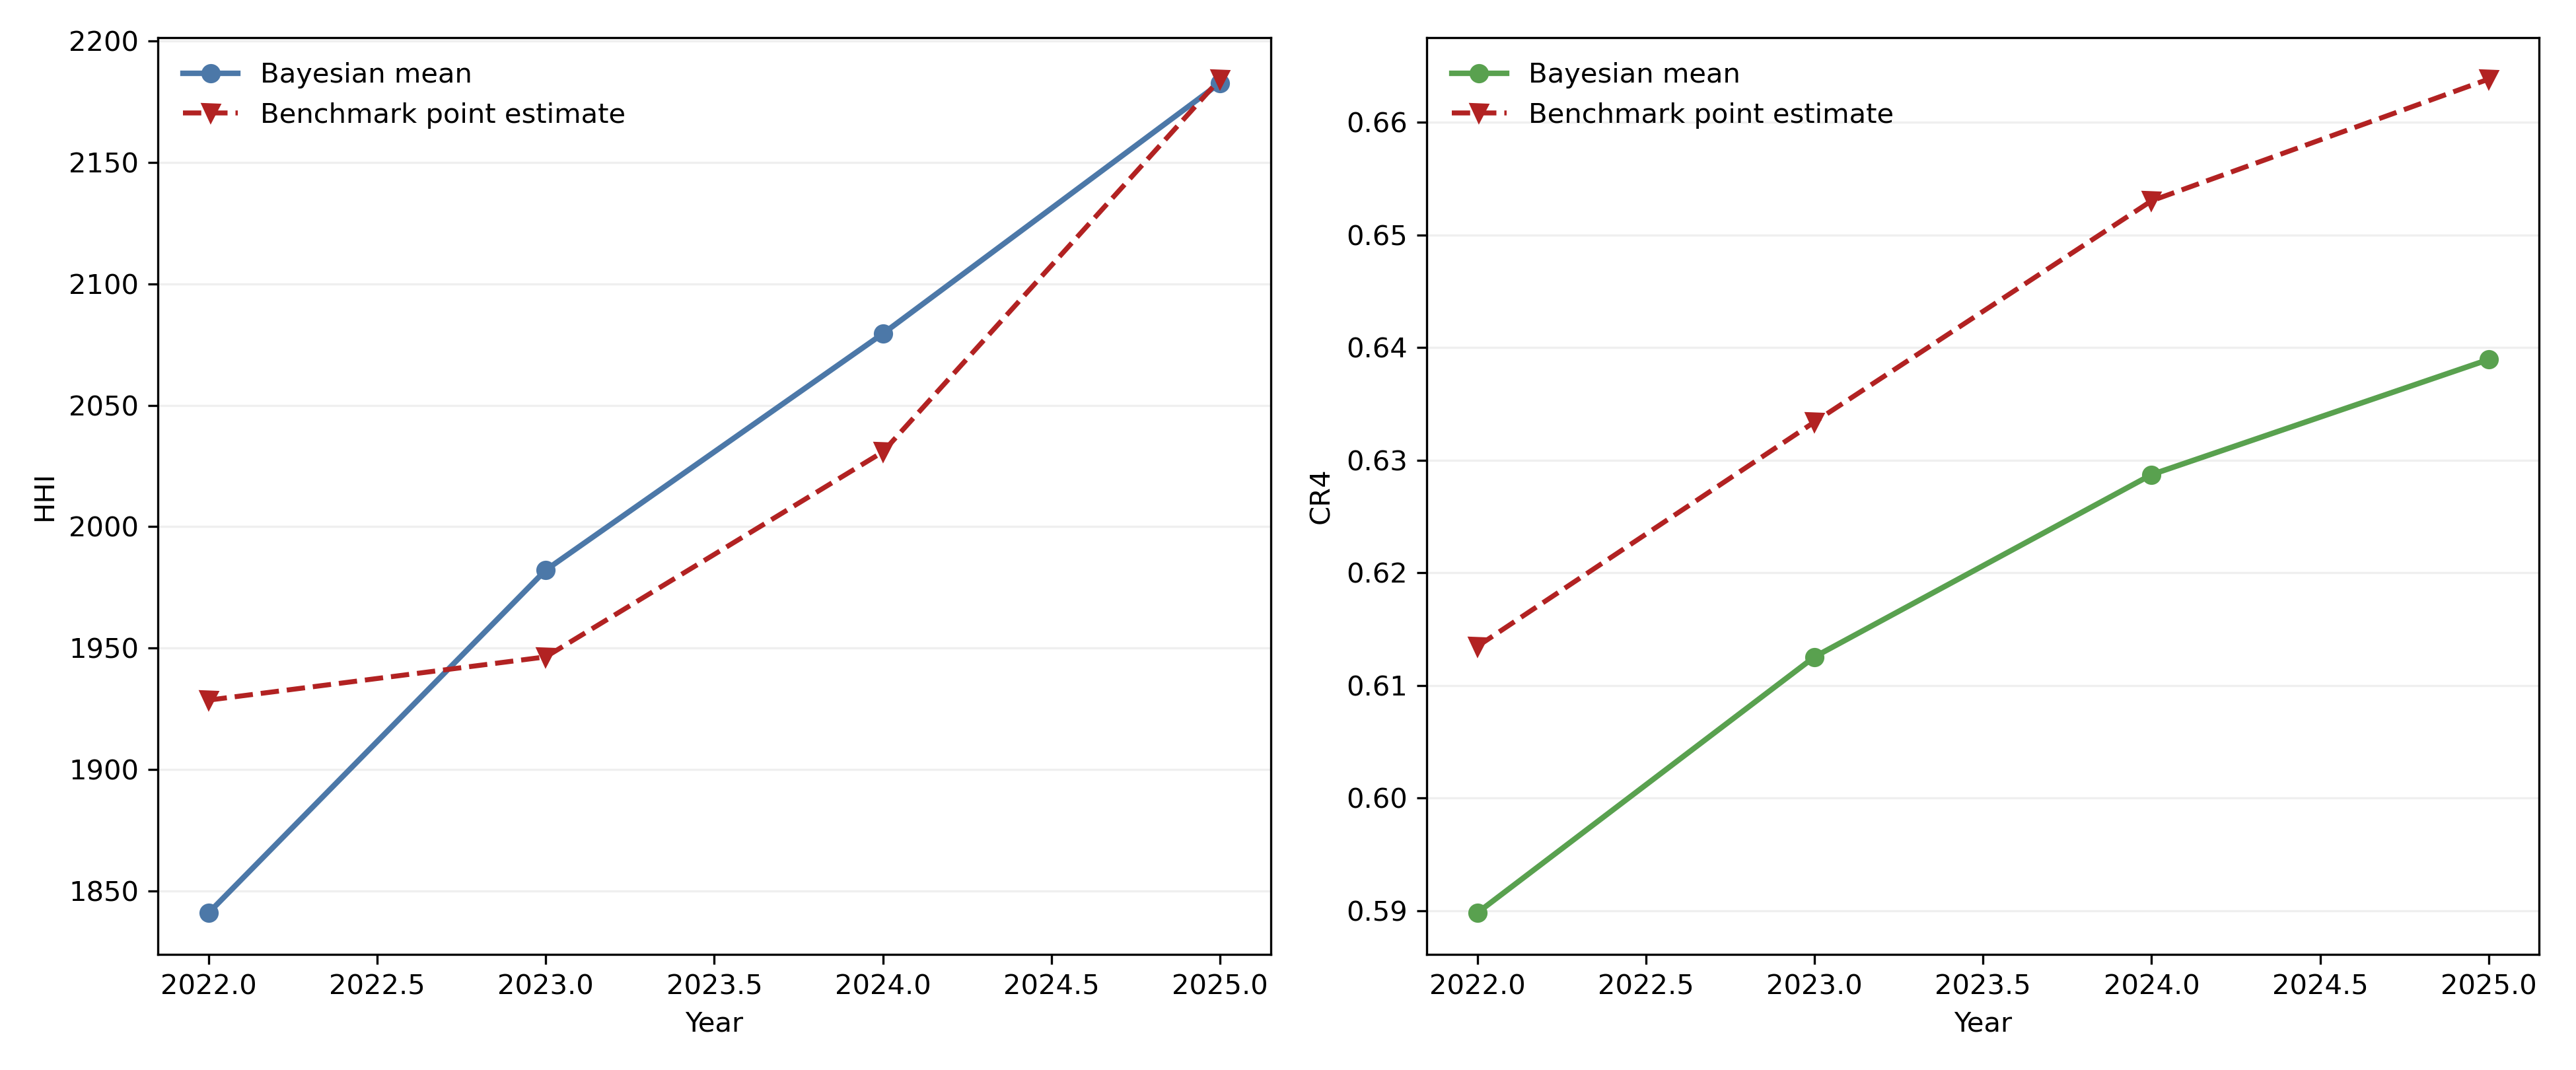
\includegraphics[width=0.92\textwidth]{../assets/figures/wrds/aggregate_concentration_trends_level_year_weighted.png}
  \end{center}

  \vspace{-0.3em}
  \small Solid (circles): Bayesian posterior mean. Dashed (triangles): benchmark. \textbf{Left:} HHI 1{,}850$\to$2{,}180. \textbf{Right:} CR4 0.59$\to$0.64.

\end{frame}

% ================================================
% POSTERIOR
% ================================================

\begin{frame}{Benchmark Overstates 2025 Concentration}

  \begin{columns}[T]
    \begin{column}{0.50\textwidth}
      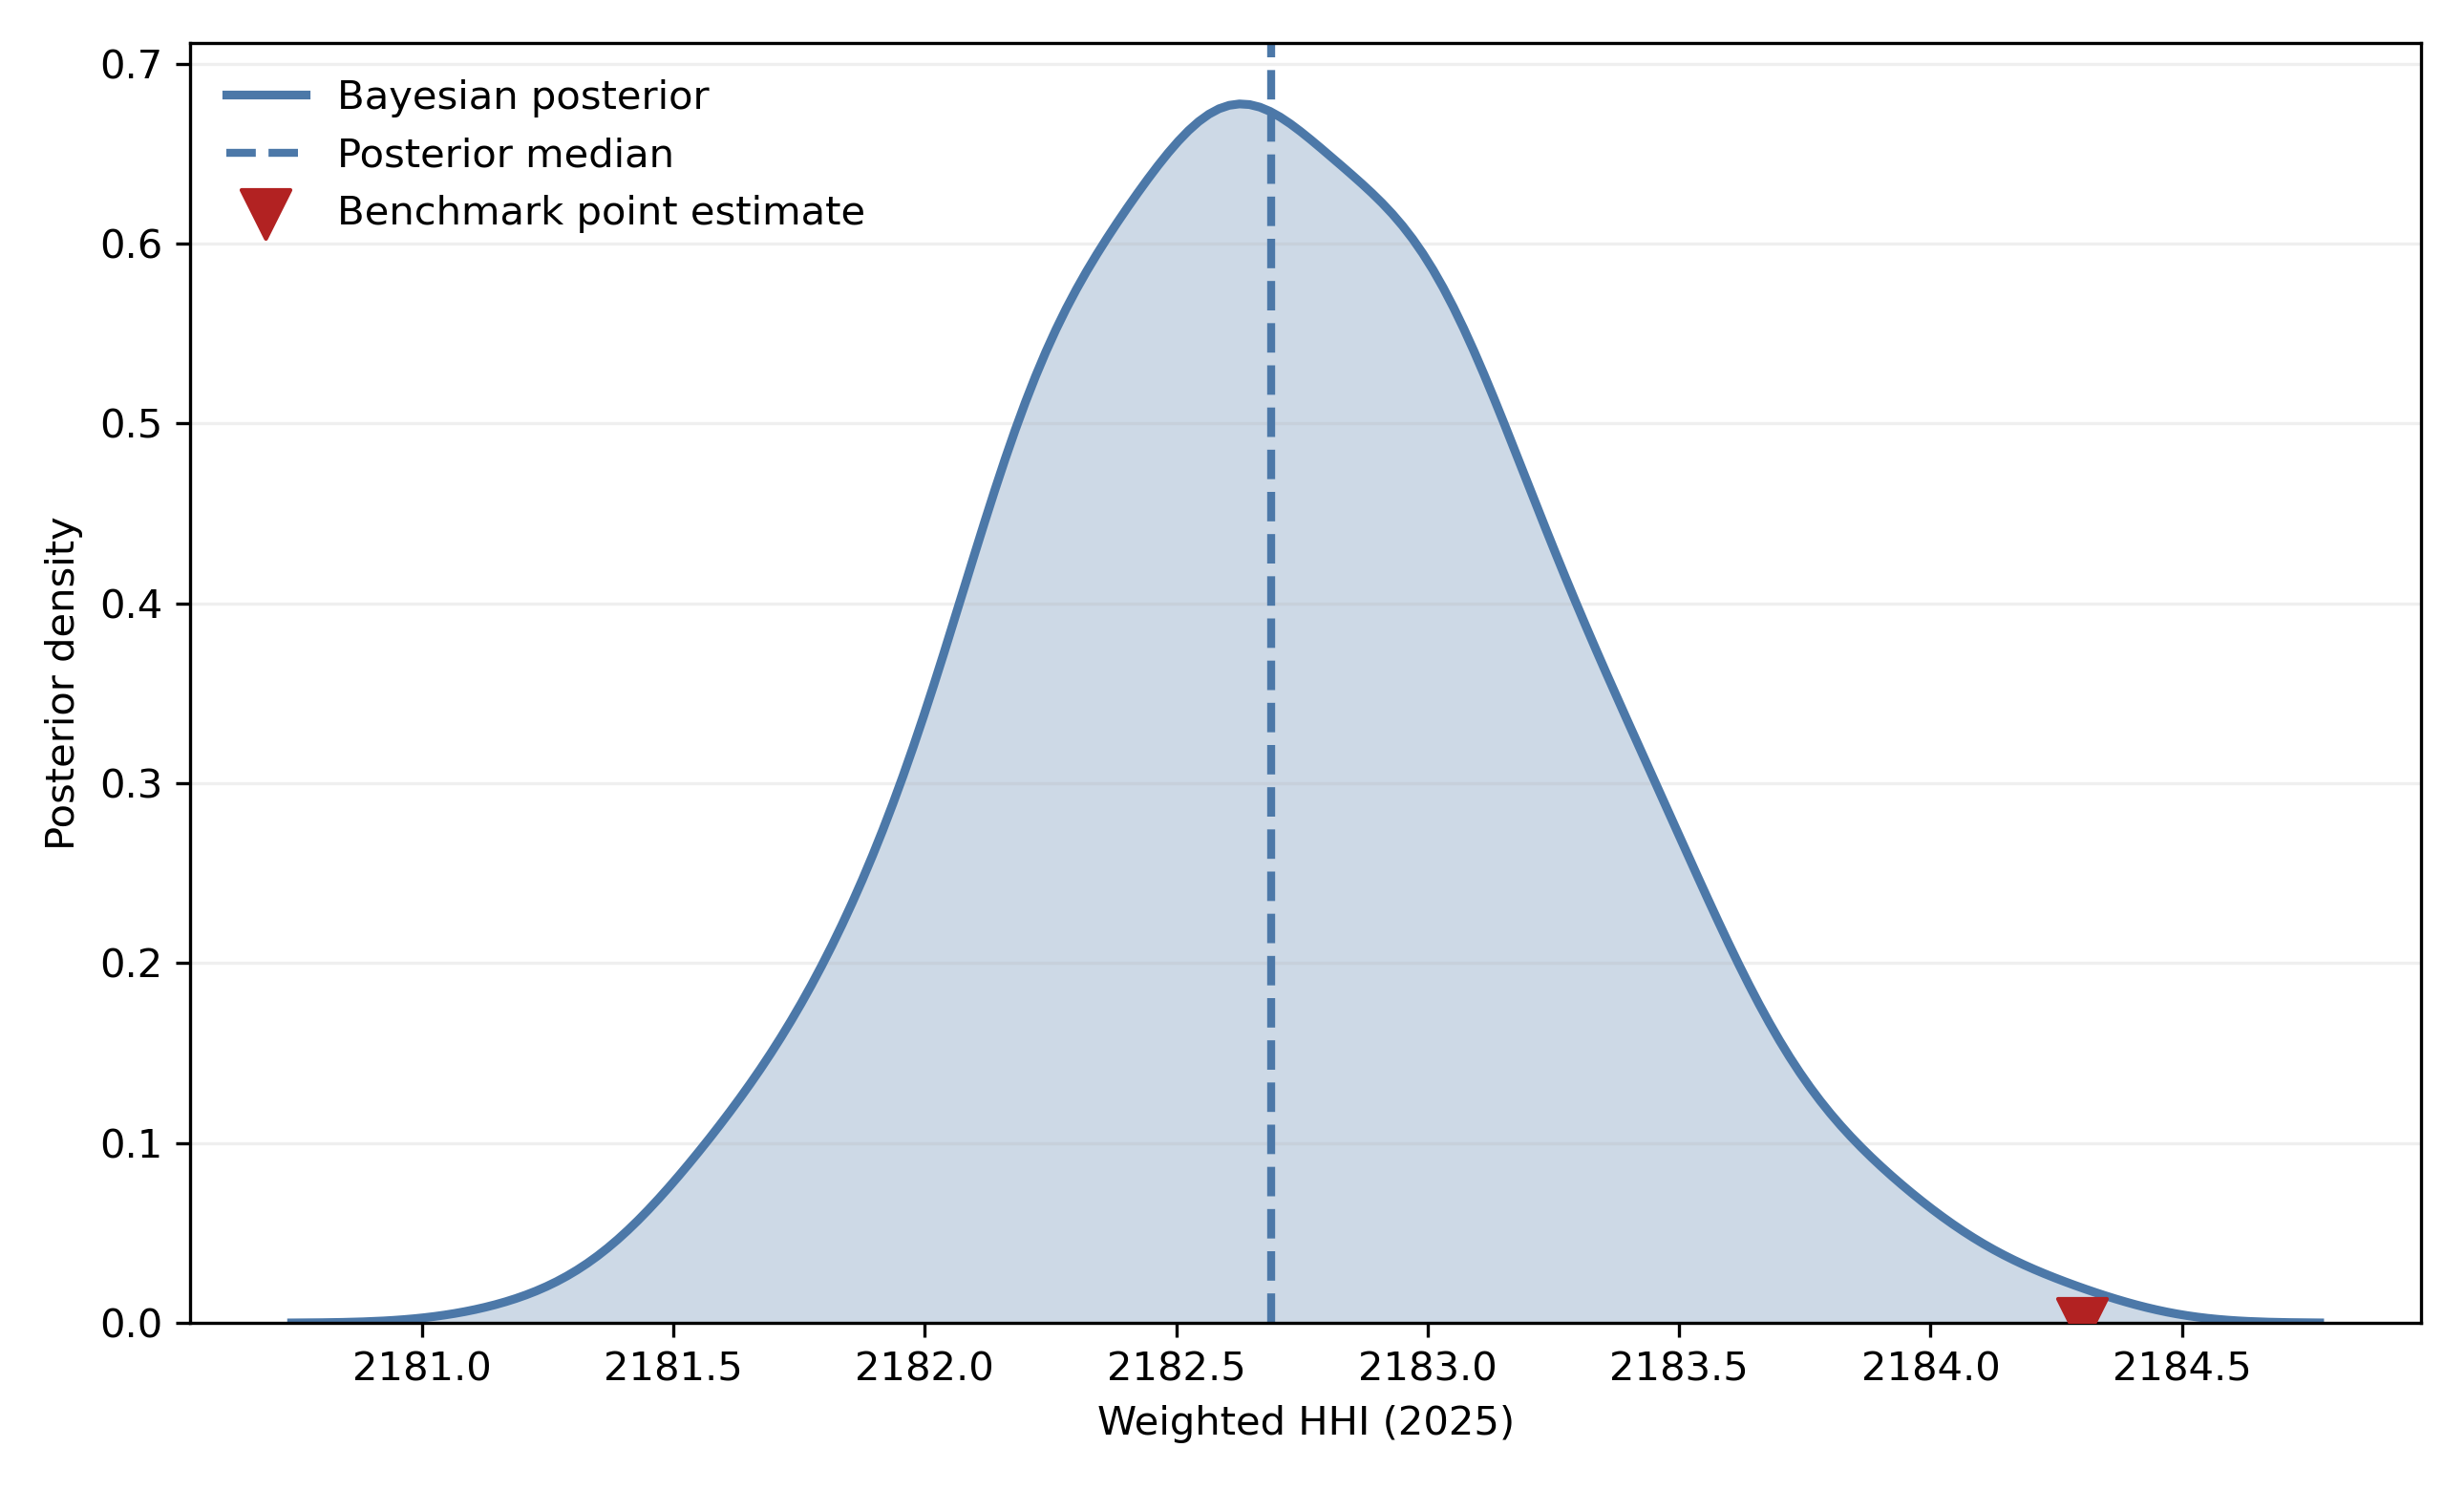
\includegraphics[width=\linewidth]{../assets/figures/wrds/hhi_distribution_2025.png}
    \end{column}
    \begin{column}{0.47\textwidth}
      \vspace{0.5em}
      \begin{alertblock}{Finding}
        Benchmark ($\approx$2{,}184.5, triangle) lies \textbf{right of} the posterior median ($\approx$2{,}182--2{,}183, dashed line).
      \end{alertblock}

      \vspace{0.8em}

      \textbf{Why?} Fixed weights place revenue in modal NAICS code\\
      $\to$ over-concentrates sales for leading firms\\
      $\to$ inflates HHI and CR4 systematically

      \vspace{0.8em}

      \textbf{Posterior is tight} ($\pm$1.5 HHI units)\\
      $\to$ gap is bias, not simulation noise
    \end{column}
  \end{columns}

\end{frame}

% ================================================
% SCATTER: BENCHMARK VS BAYESIAN BY INDUSTRY
% ================================================

\begin{frame}{Benchmark Overstates Across Industries (2025)}

  \begin{columns}[T]
    \begin{column}{0.48\textwidth}
      \centering
      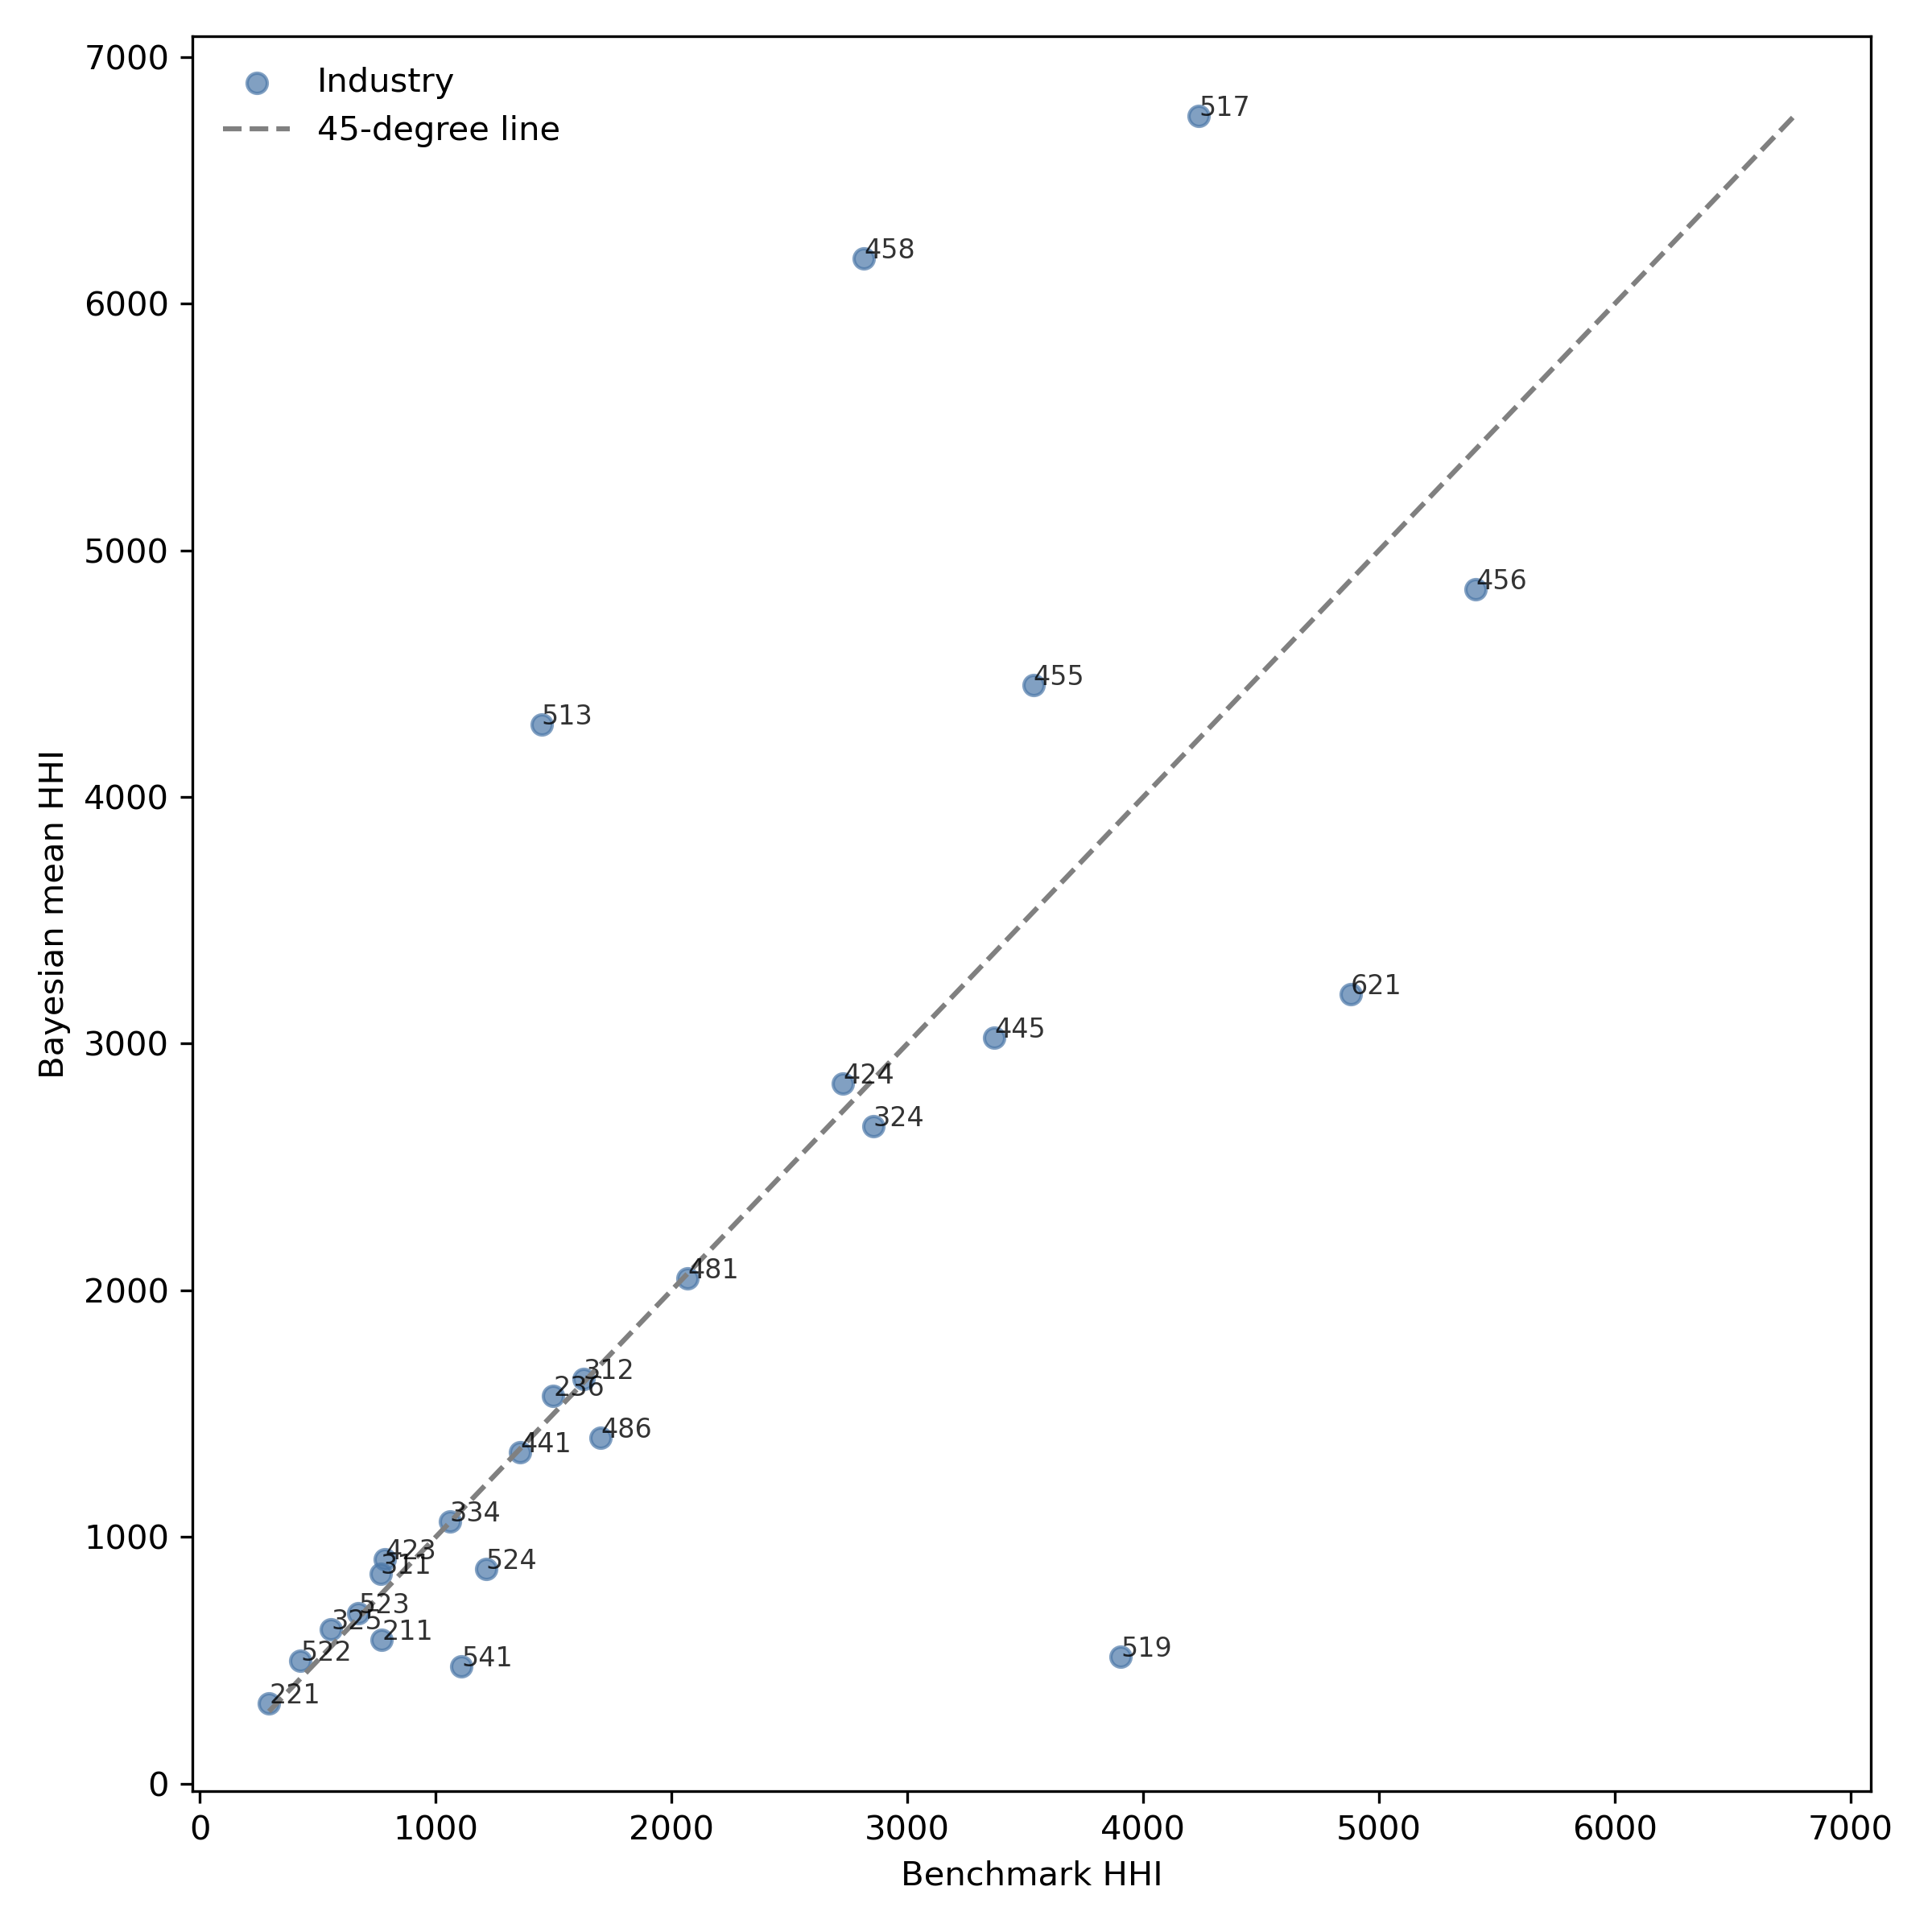
\includegraphics[width=\linewidth]{../assets/figures/wrds/hhi_scatter_comparison_2025.png}
      \small HHI
    \end{column}
    \begin{column}{0.48\textwidth}
      \centering
      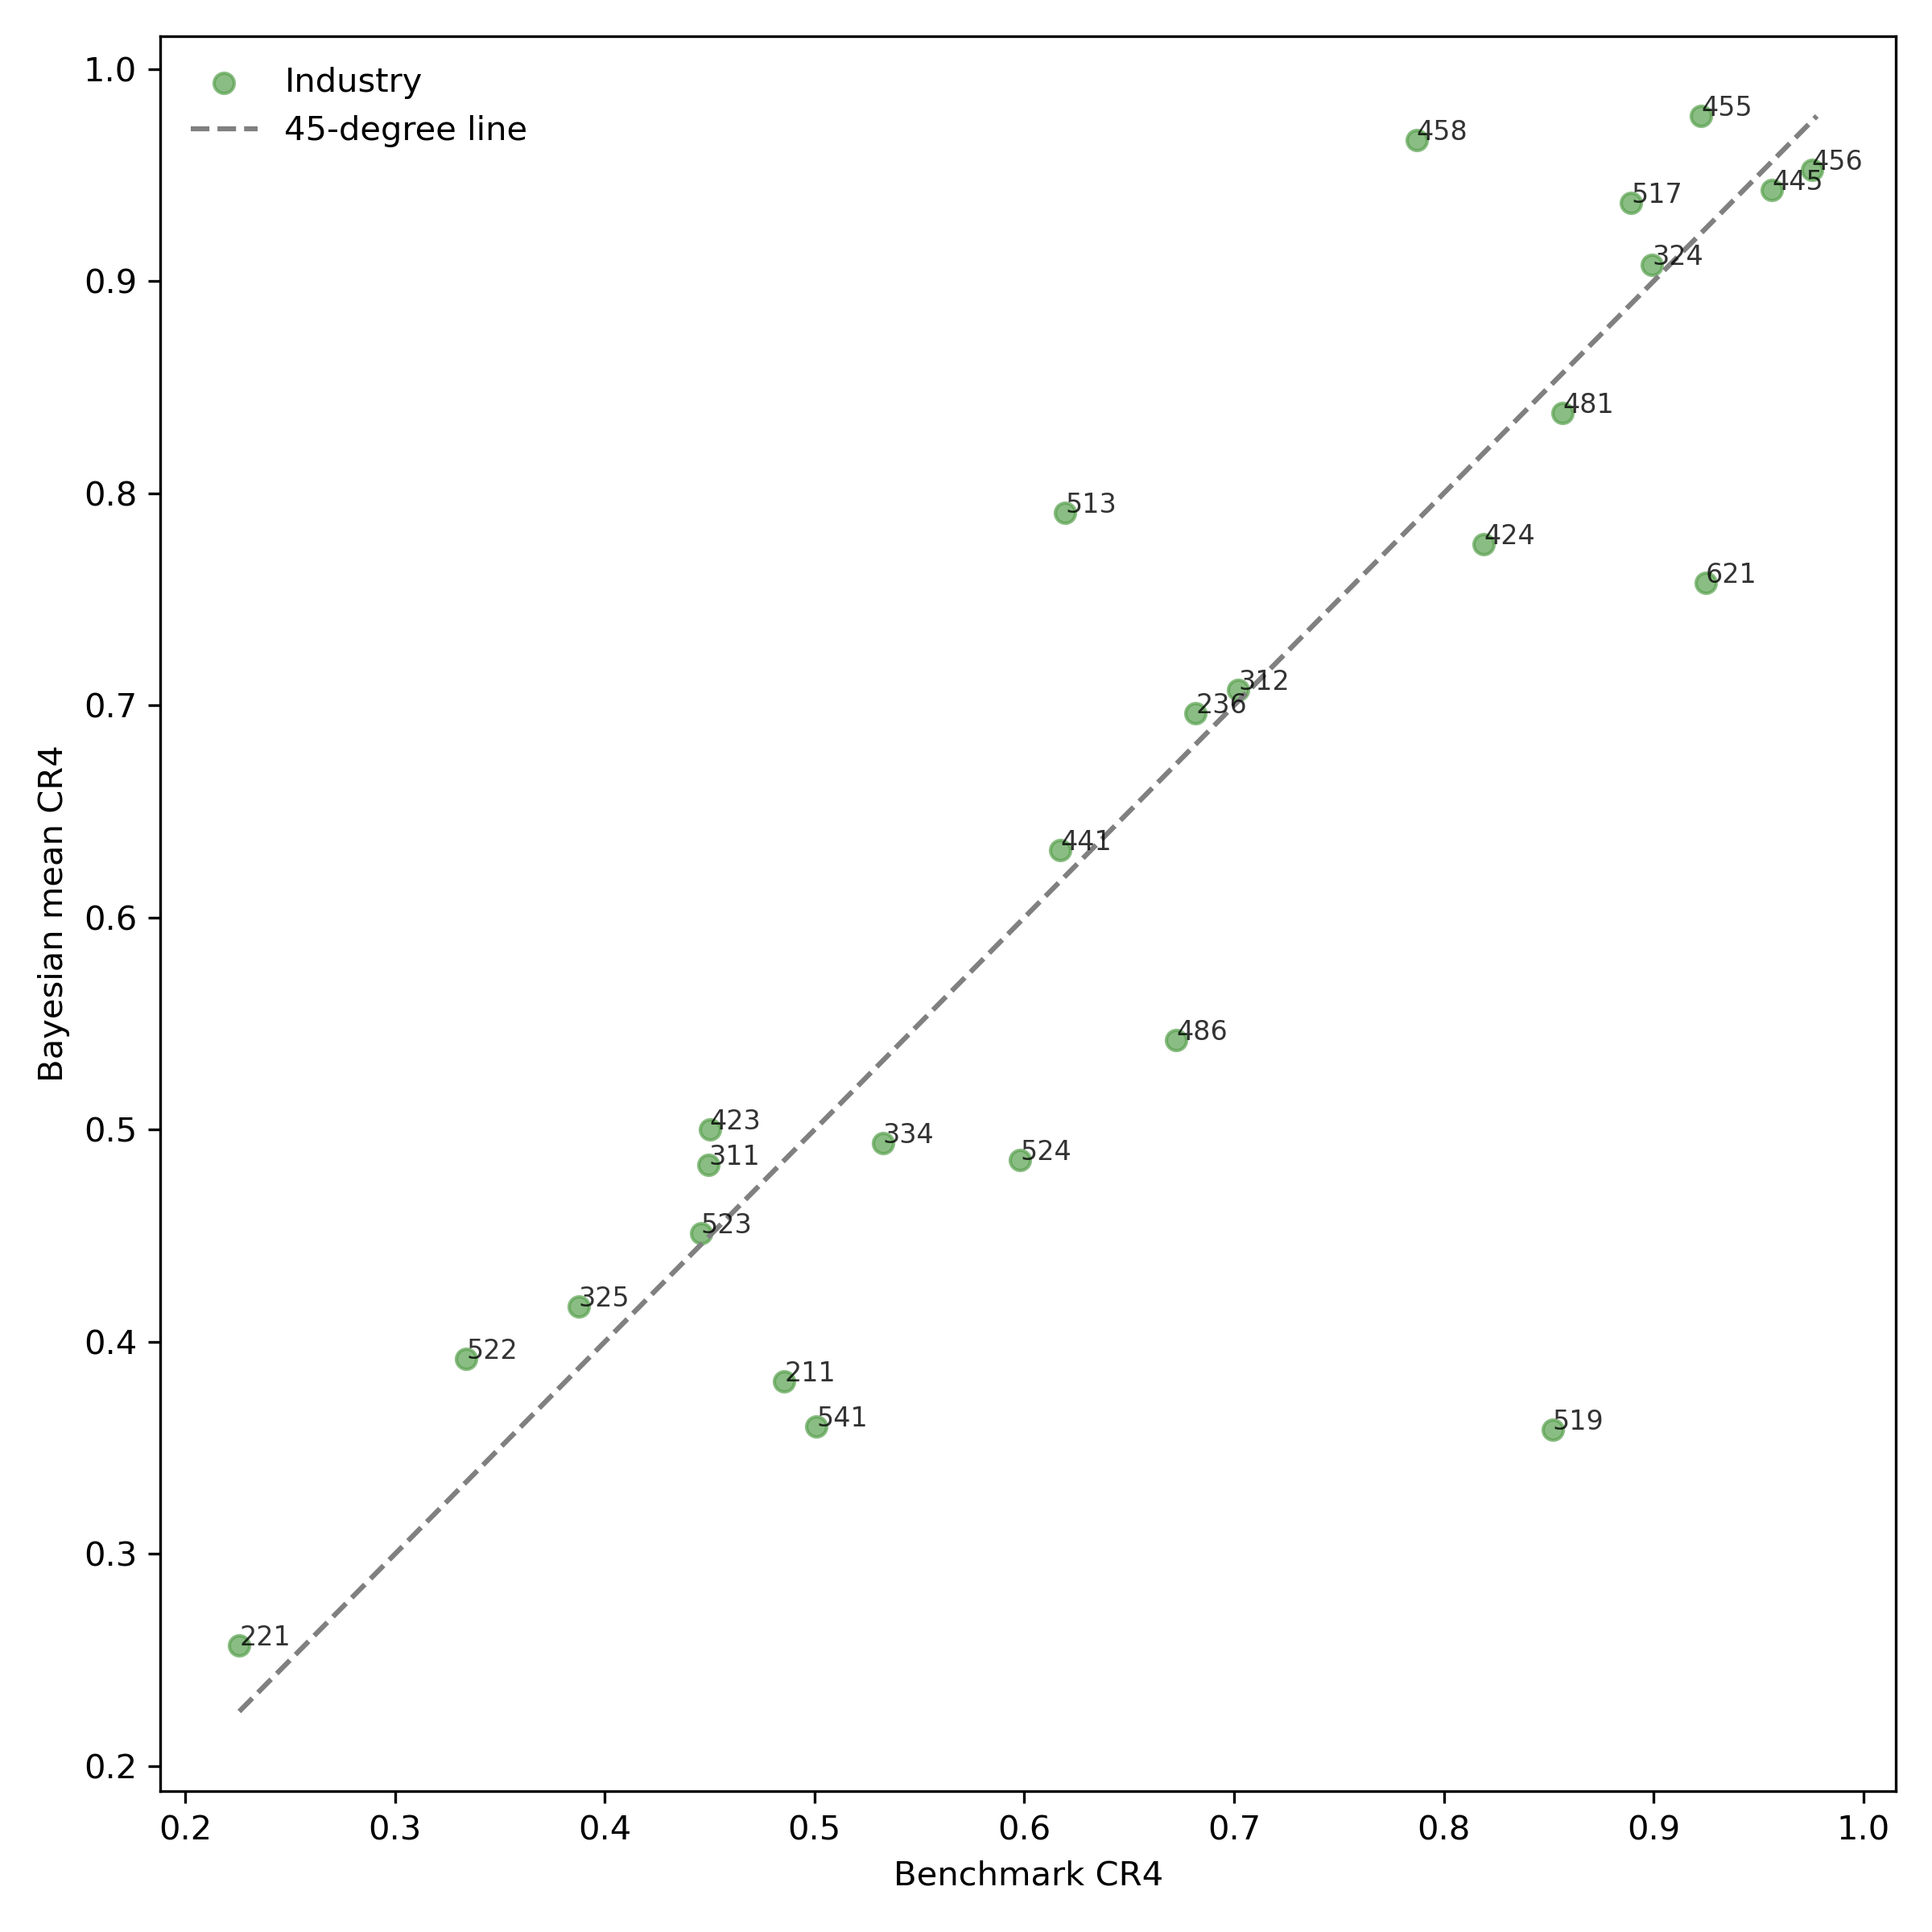
\includegraphics[width=\linewidth]{../assets/figures/wrds/cr4_scatter_comparison_2025.png}
      \small CR4
    \end{column}
  \end{columns}

  \vspace{0.4em}
  \small $x$ = benchmark, $y$ = Bayesian posterior mean. Points \textbf{below} the 45-degree line: benchmark overstates concentration. Pattern holds across most 3-digit NAICS industries.

\end{frame}

% ================================================
% INDUSTRY HETEROGENEITY
% ================================================

\begin{frame}{Cross-Industry Heterogeneity in Posterior Uncertainty}

  \begin{center}
    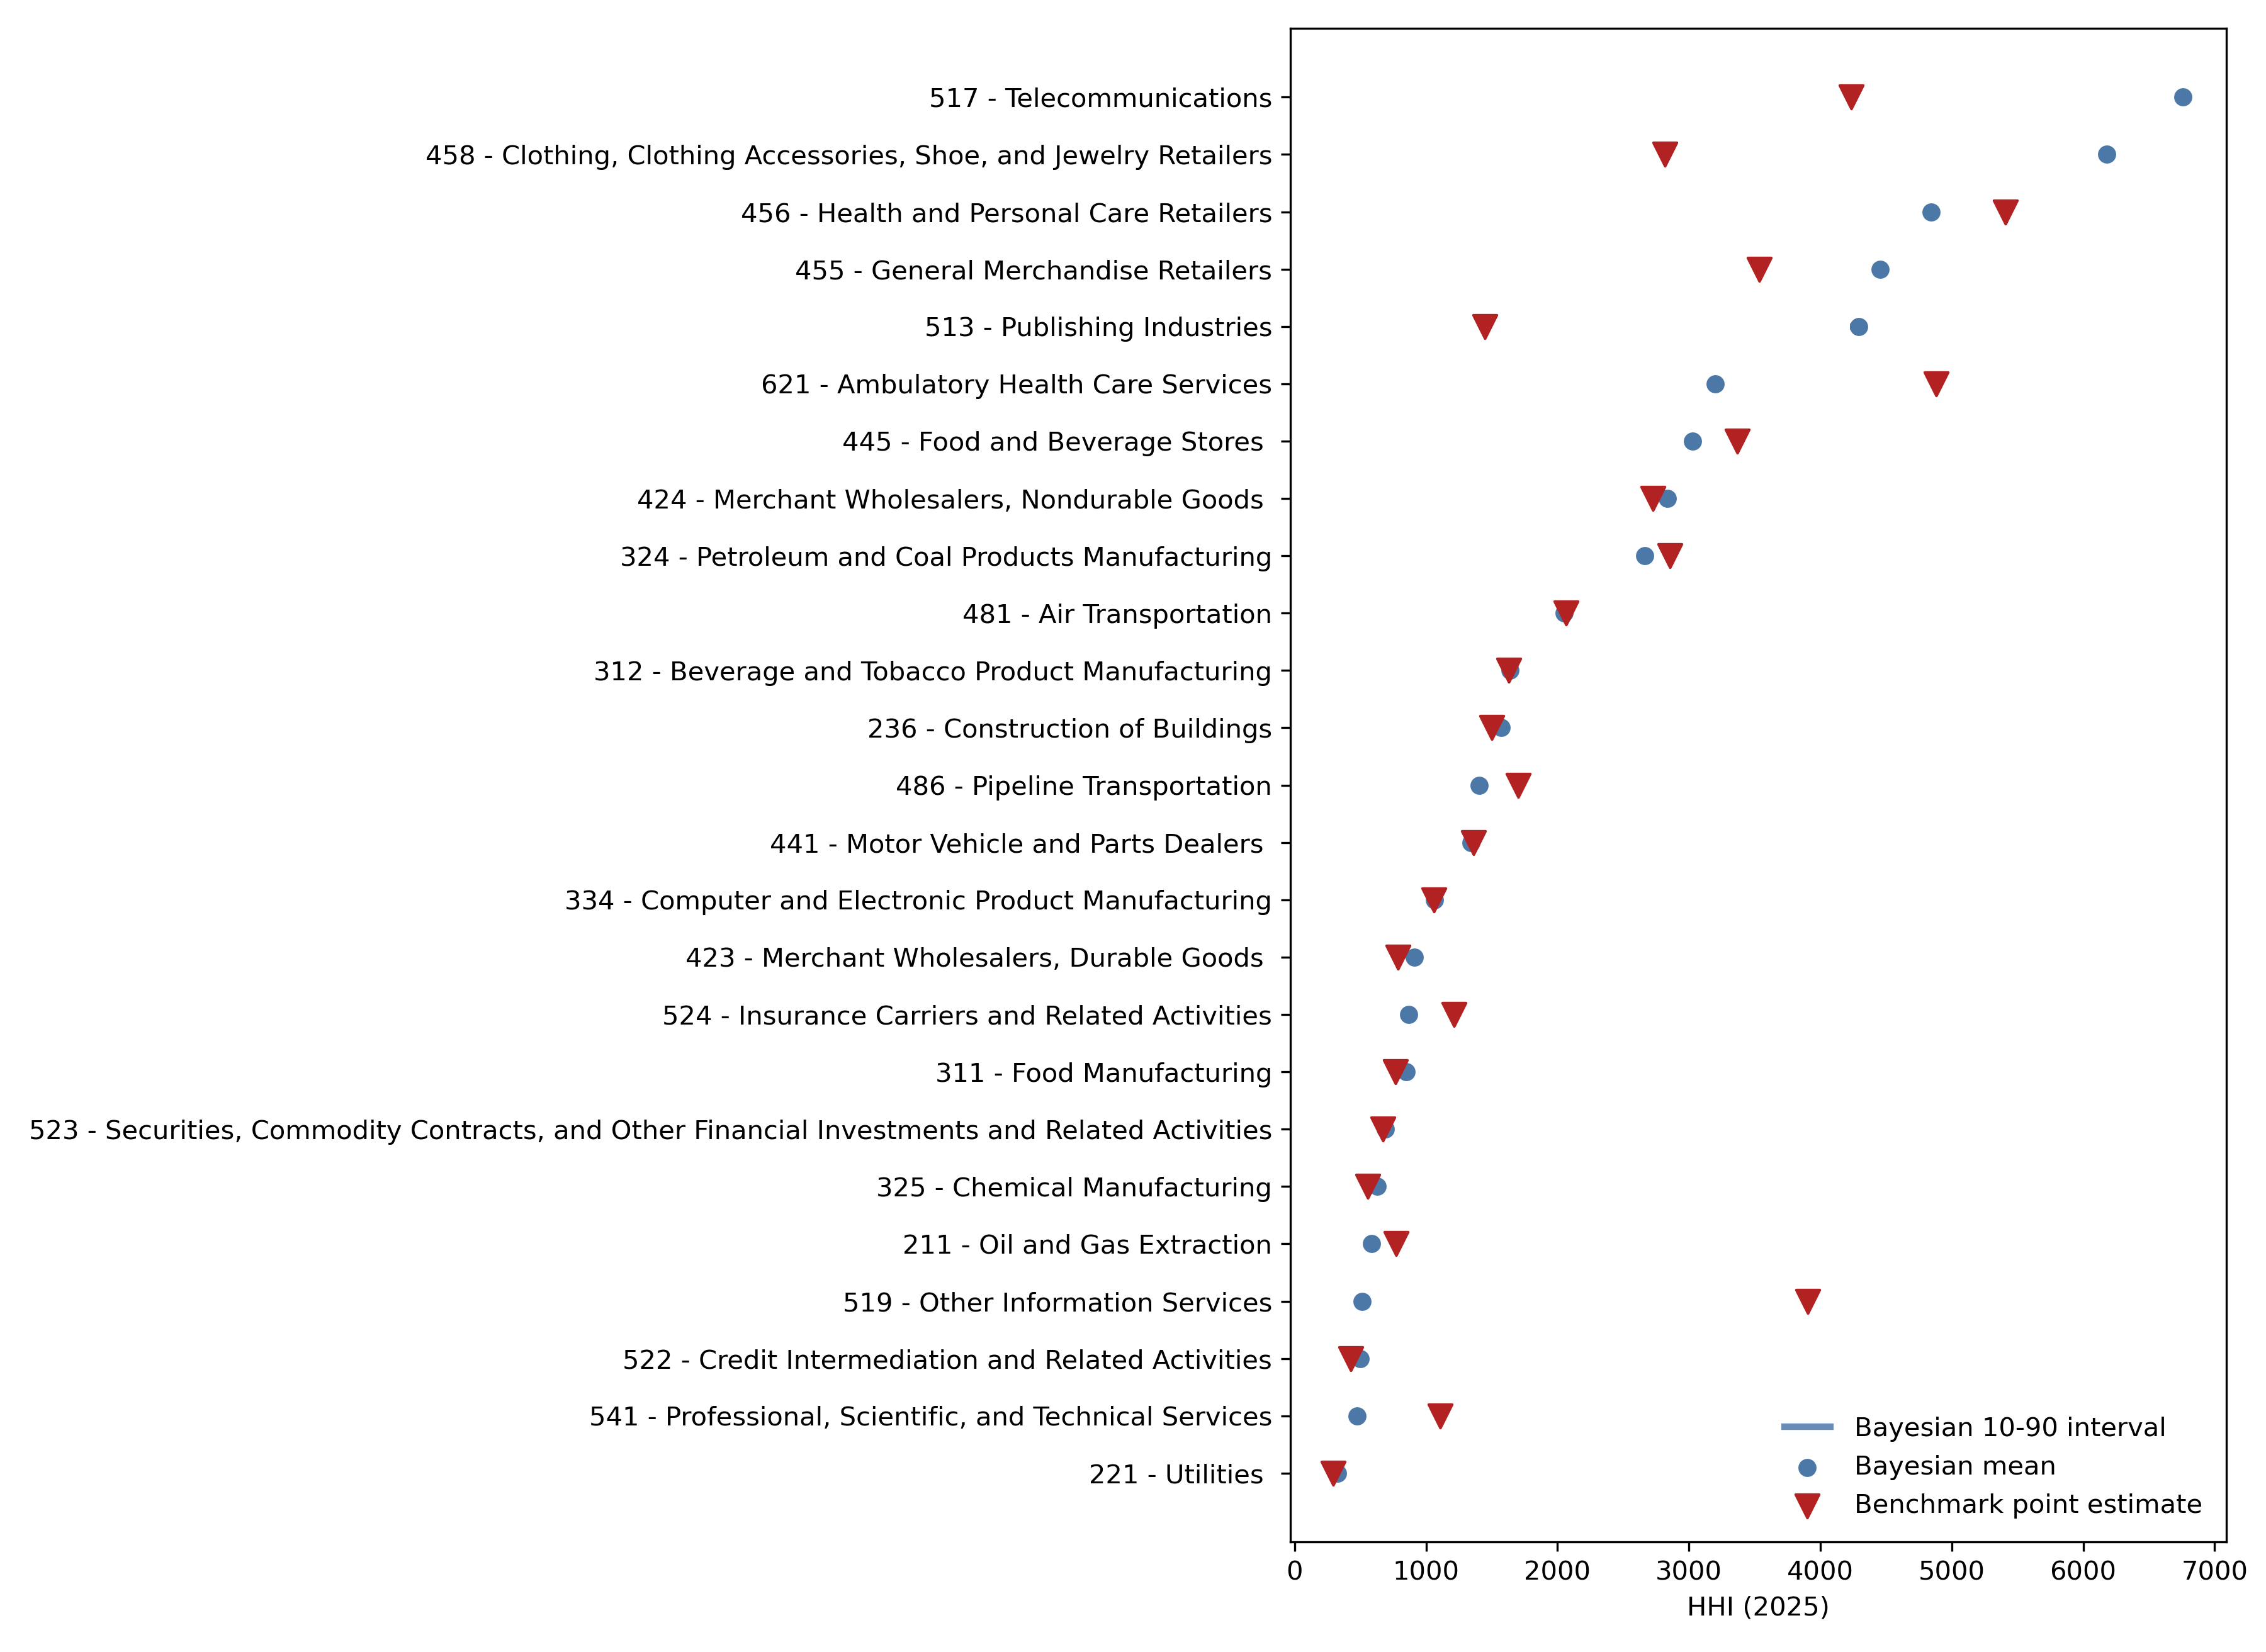
\includegraphics[width=0.6\textwidth]{../assets/figures/wrds/hhi_comparison_by_industry_2025.png}
  \end{center}


\end{frame}

% ================================================
% LOG CHANGE
% ================================================

\begin{frame}{Concentration Growth Is Robust}

  \begin{center}
    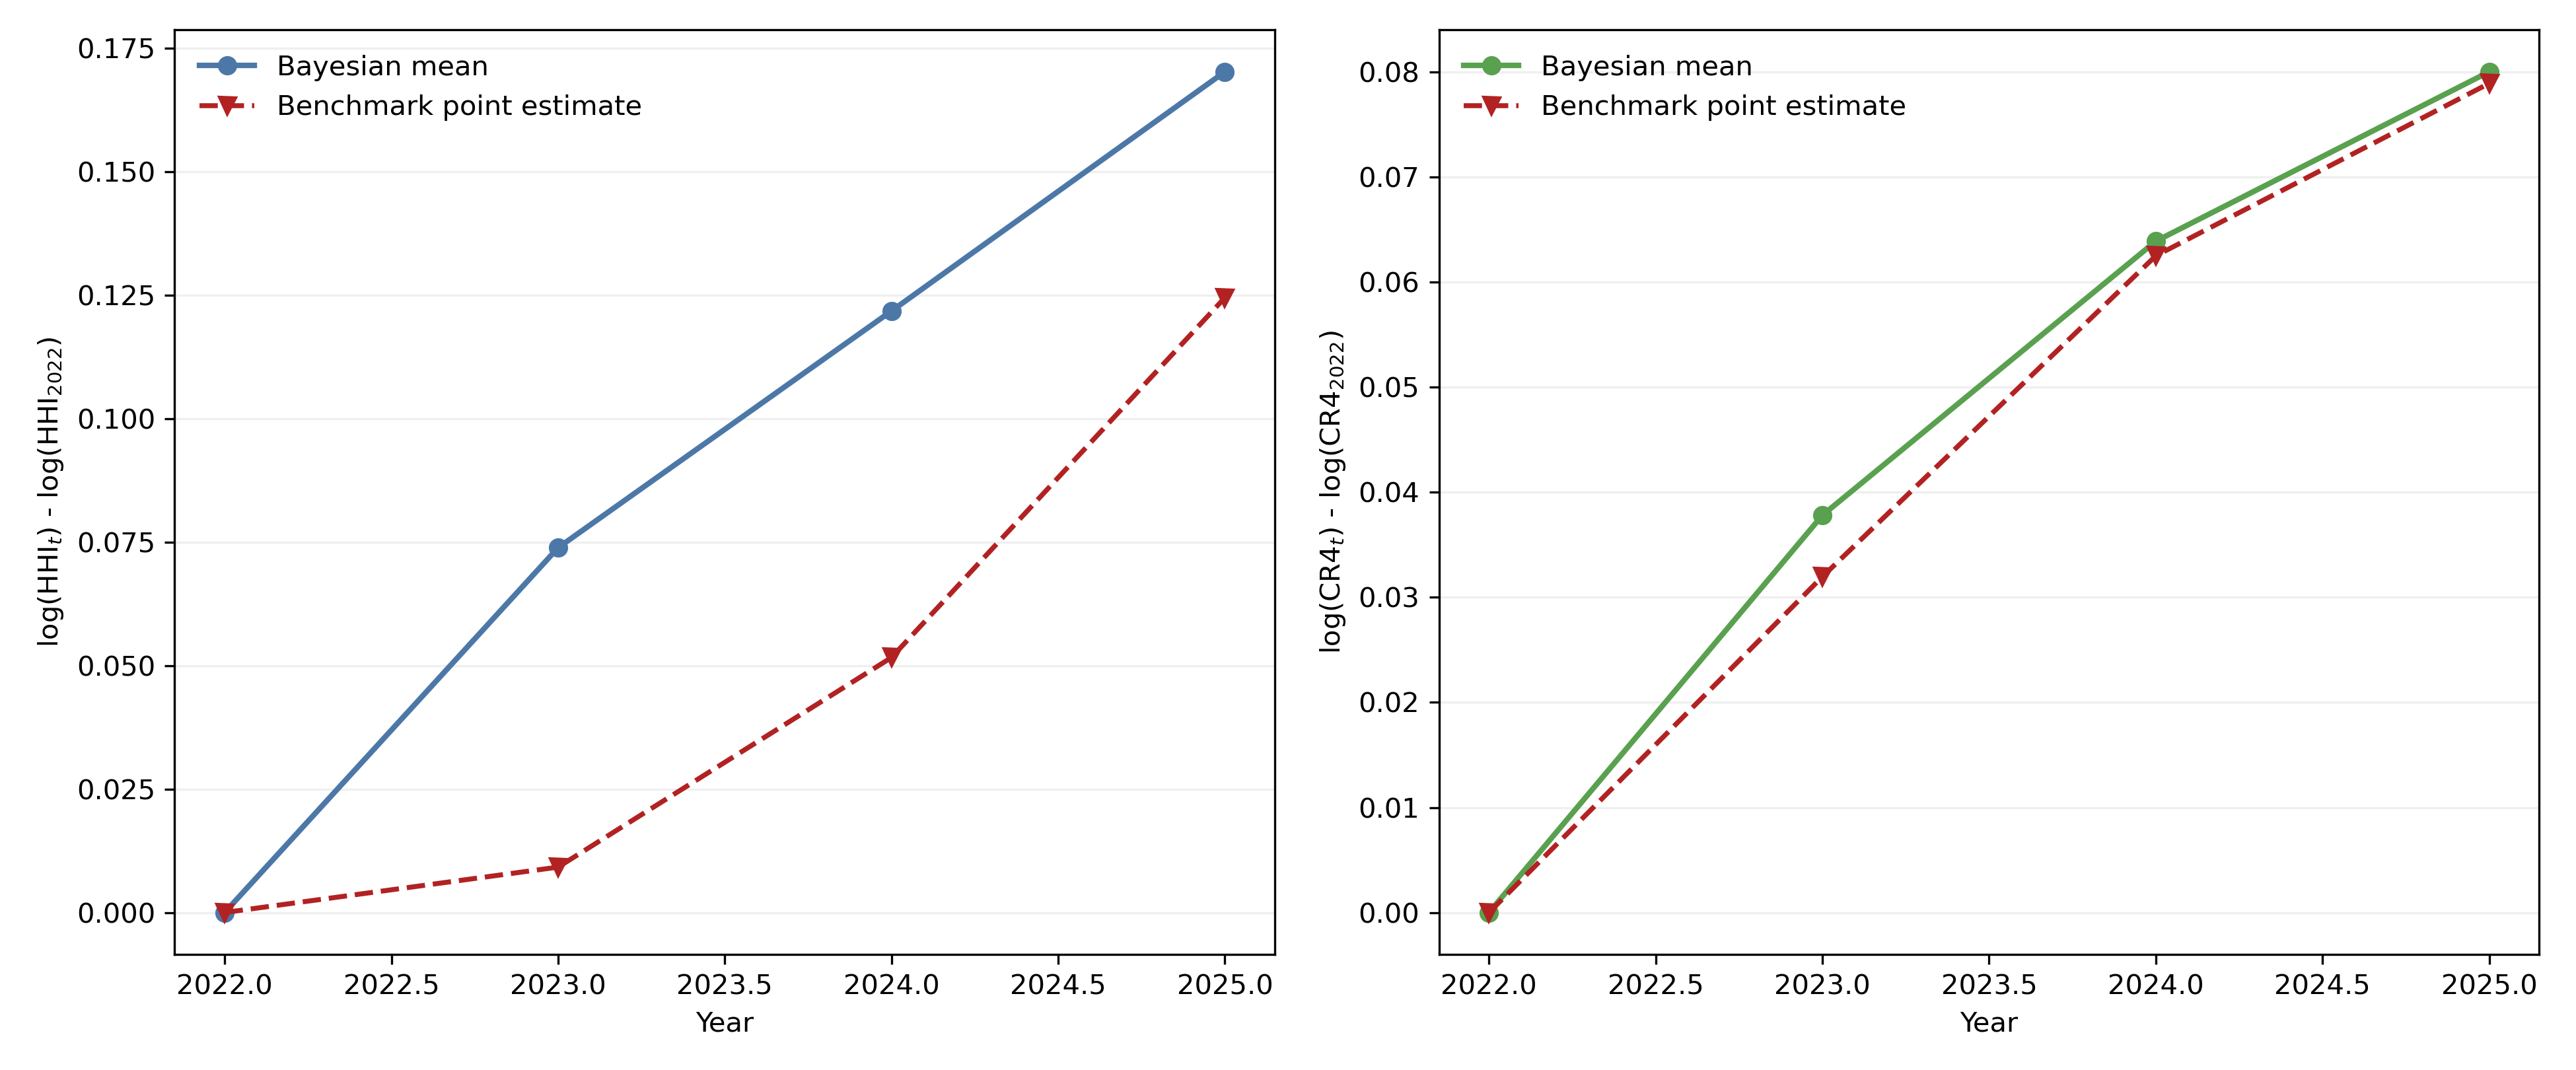
\includegraphics[width=0.85\textwidth]{../assets/figures/wrds/aggregate_concentration_trends_log_year_weighted.png}
  \end{center}

  \vspace{-0.4em}
  \small Log-change from 2022. Lower bound of 2025 credible band is above zero in every post-2022 year. Trend is structural.

\end{frame}

% ================================================
% NAICS 3-DIGIT PRELIMINARY EVIDENCE 
% ================================================

\begin{frame}{NAICS 3-Digit Evidence}

  %\textit{Ongoing analysis; consistent pattern across all industries examined so far.}

  \vspace{1em}

  \begin{block}{Finding 1: CR4 is more distorted than HHI}
    Traditional HHI point estimates fall closer to---and more often within---the Bayesian HHI posterior than traditional CR4 estimates do to the Bayesian CR4 posterior.

    \medskip
    \textbf{Why:} CR4 is a rank statistic. Small allocation shifts can reshuffle the top-four; HHI is a smooth quadratic---more robust to rank permutations.
  \end{block}

  \vspace{0.8em}

  \begin{alertblock}{Finding 2: Benchmark overstates levels but understates growth}
    Fixed-assignment measures overstate concentration \textbf{today} and understate how fast it is rising.

    \medskip
    \textbf{Why:} In the data, the Bayesian series starts from a lower baseline and rises faster. One interpretation is that ambiguous segment revenue is initially allocated more diffusely and then shifts toward dominant firms as later-year evidence accumulates. The deterministic benchmark collapses each year to one fixed allocation vector, so it misses this intertemporal uncertainty margin.
  \end{alertblock}

\end{frame}

% ================================================
% TAKEAWAYS
% ================================================

\begin{frame}{Takeaways}

  \begin{enumerate}
    \setlength\itemsep{0.6em}
    \item \textbf{Concentration has risen sharply post COVID.}
          Sales-weighted HHI up 330 points (18\%) from 2022 to 2025.

    \item \textbf{Standard measures overstate concentration levels.}
          Benchmark sits in the right tail of the Bayesian posterior---systematic bias, not noise.

    \item \textbf{\ldots but understate concentration growth.}
          Fixed yearly assignment misses the steeper trend the Bayesian model reveals once allocation uncertainty is propagated over time.

    \item \textbf{CR4 is more distorted than HHI.}
          Rank-order sensitivity makes CR4 more susceptible to small allocation shifts.

    \item \textbf{Both errors matter for measuring competition.}
          Over-intervention today,  under-intervention for growth over time.
  \end{enumerate}

  \vfill

  %\small\textit{Next: complete NAICS 3-digit sweep; validate against NielsenIQ/Numerator; compute $P(\mathrm{HHI} > 2{,}500)$ by industry.}

\end{frame}

% ================================================
% APPENDIX
% ================================================

\appendix

\begin{frame}[noframenumbering]{Appendix: Segment-Level Dirichlet Posterior}

  \begin{center}
    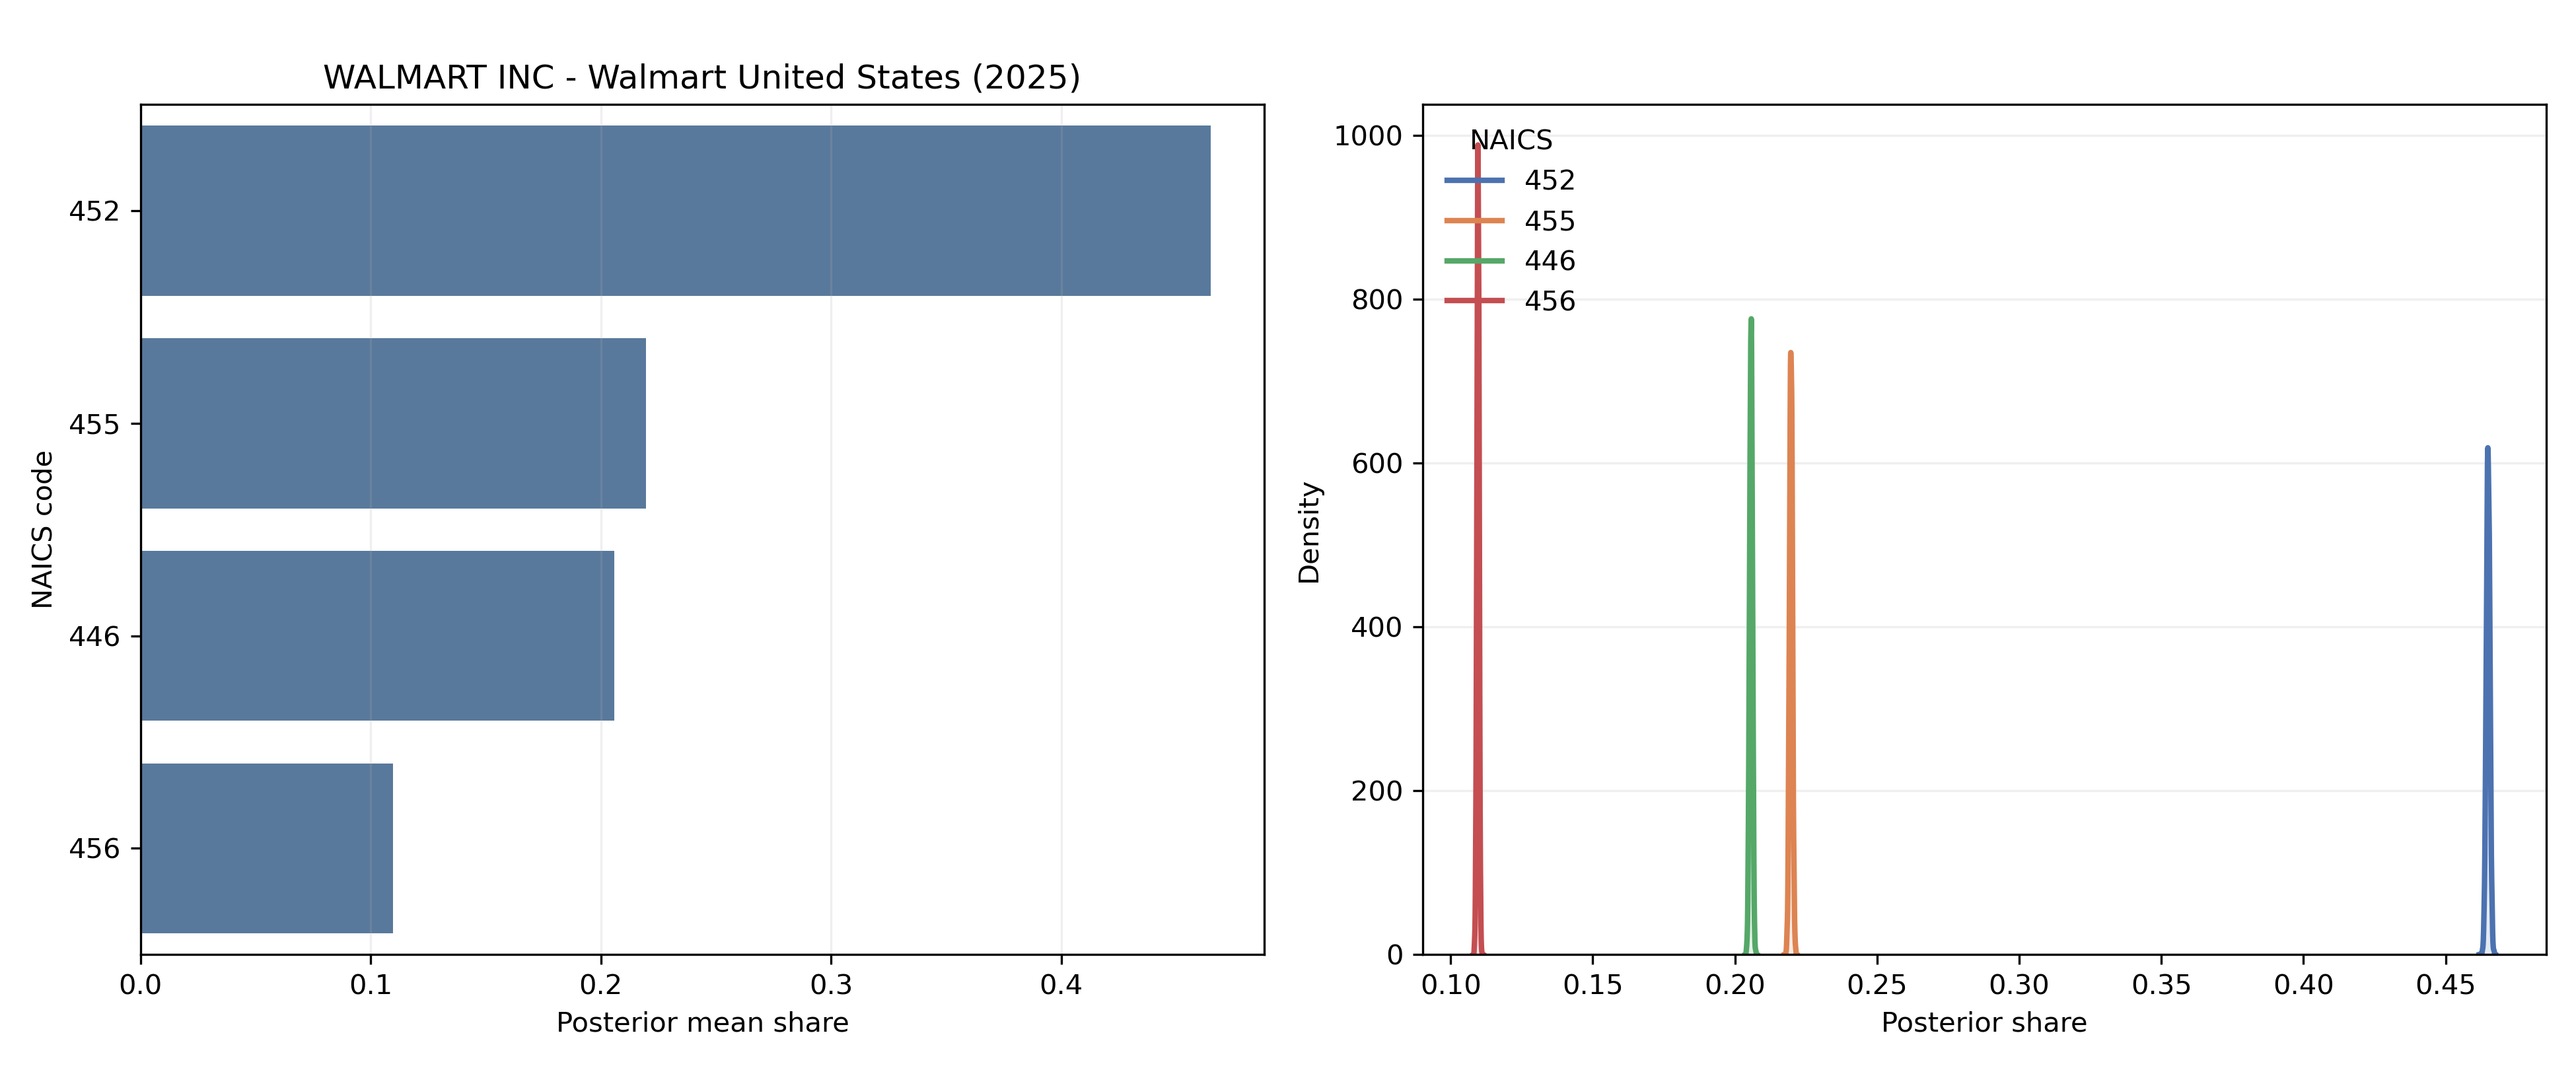
\includegraphics[width=0.75\textwidth]{../assets/figures/wrds/dirichlet_posterior_example_2025.png}
  \end{center}

  \vspace{-0.3em}
  \small Posterior allocation for a single large 2025 segment with $\geq$3 NAICS links. Meaningful within-segment uncertainty even with an informative prior.

\end{frame}


\begin{frame}[noframenumbering]{Appendix: CR4 by Industry, 2025}

  \begin{center}
    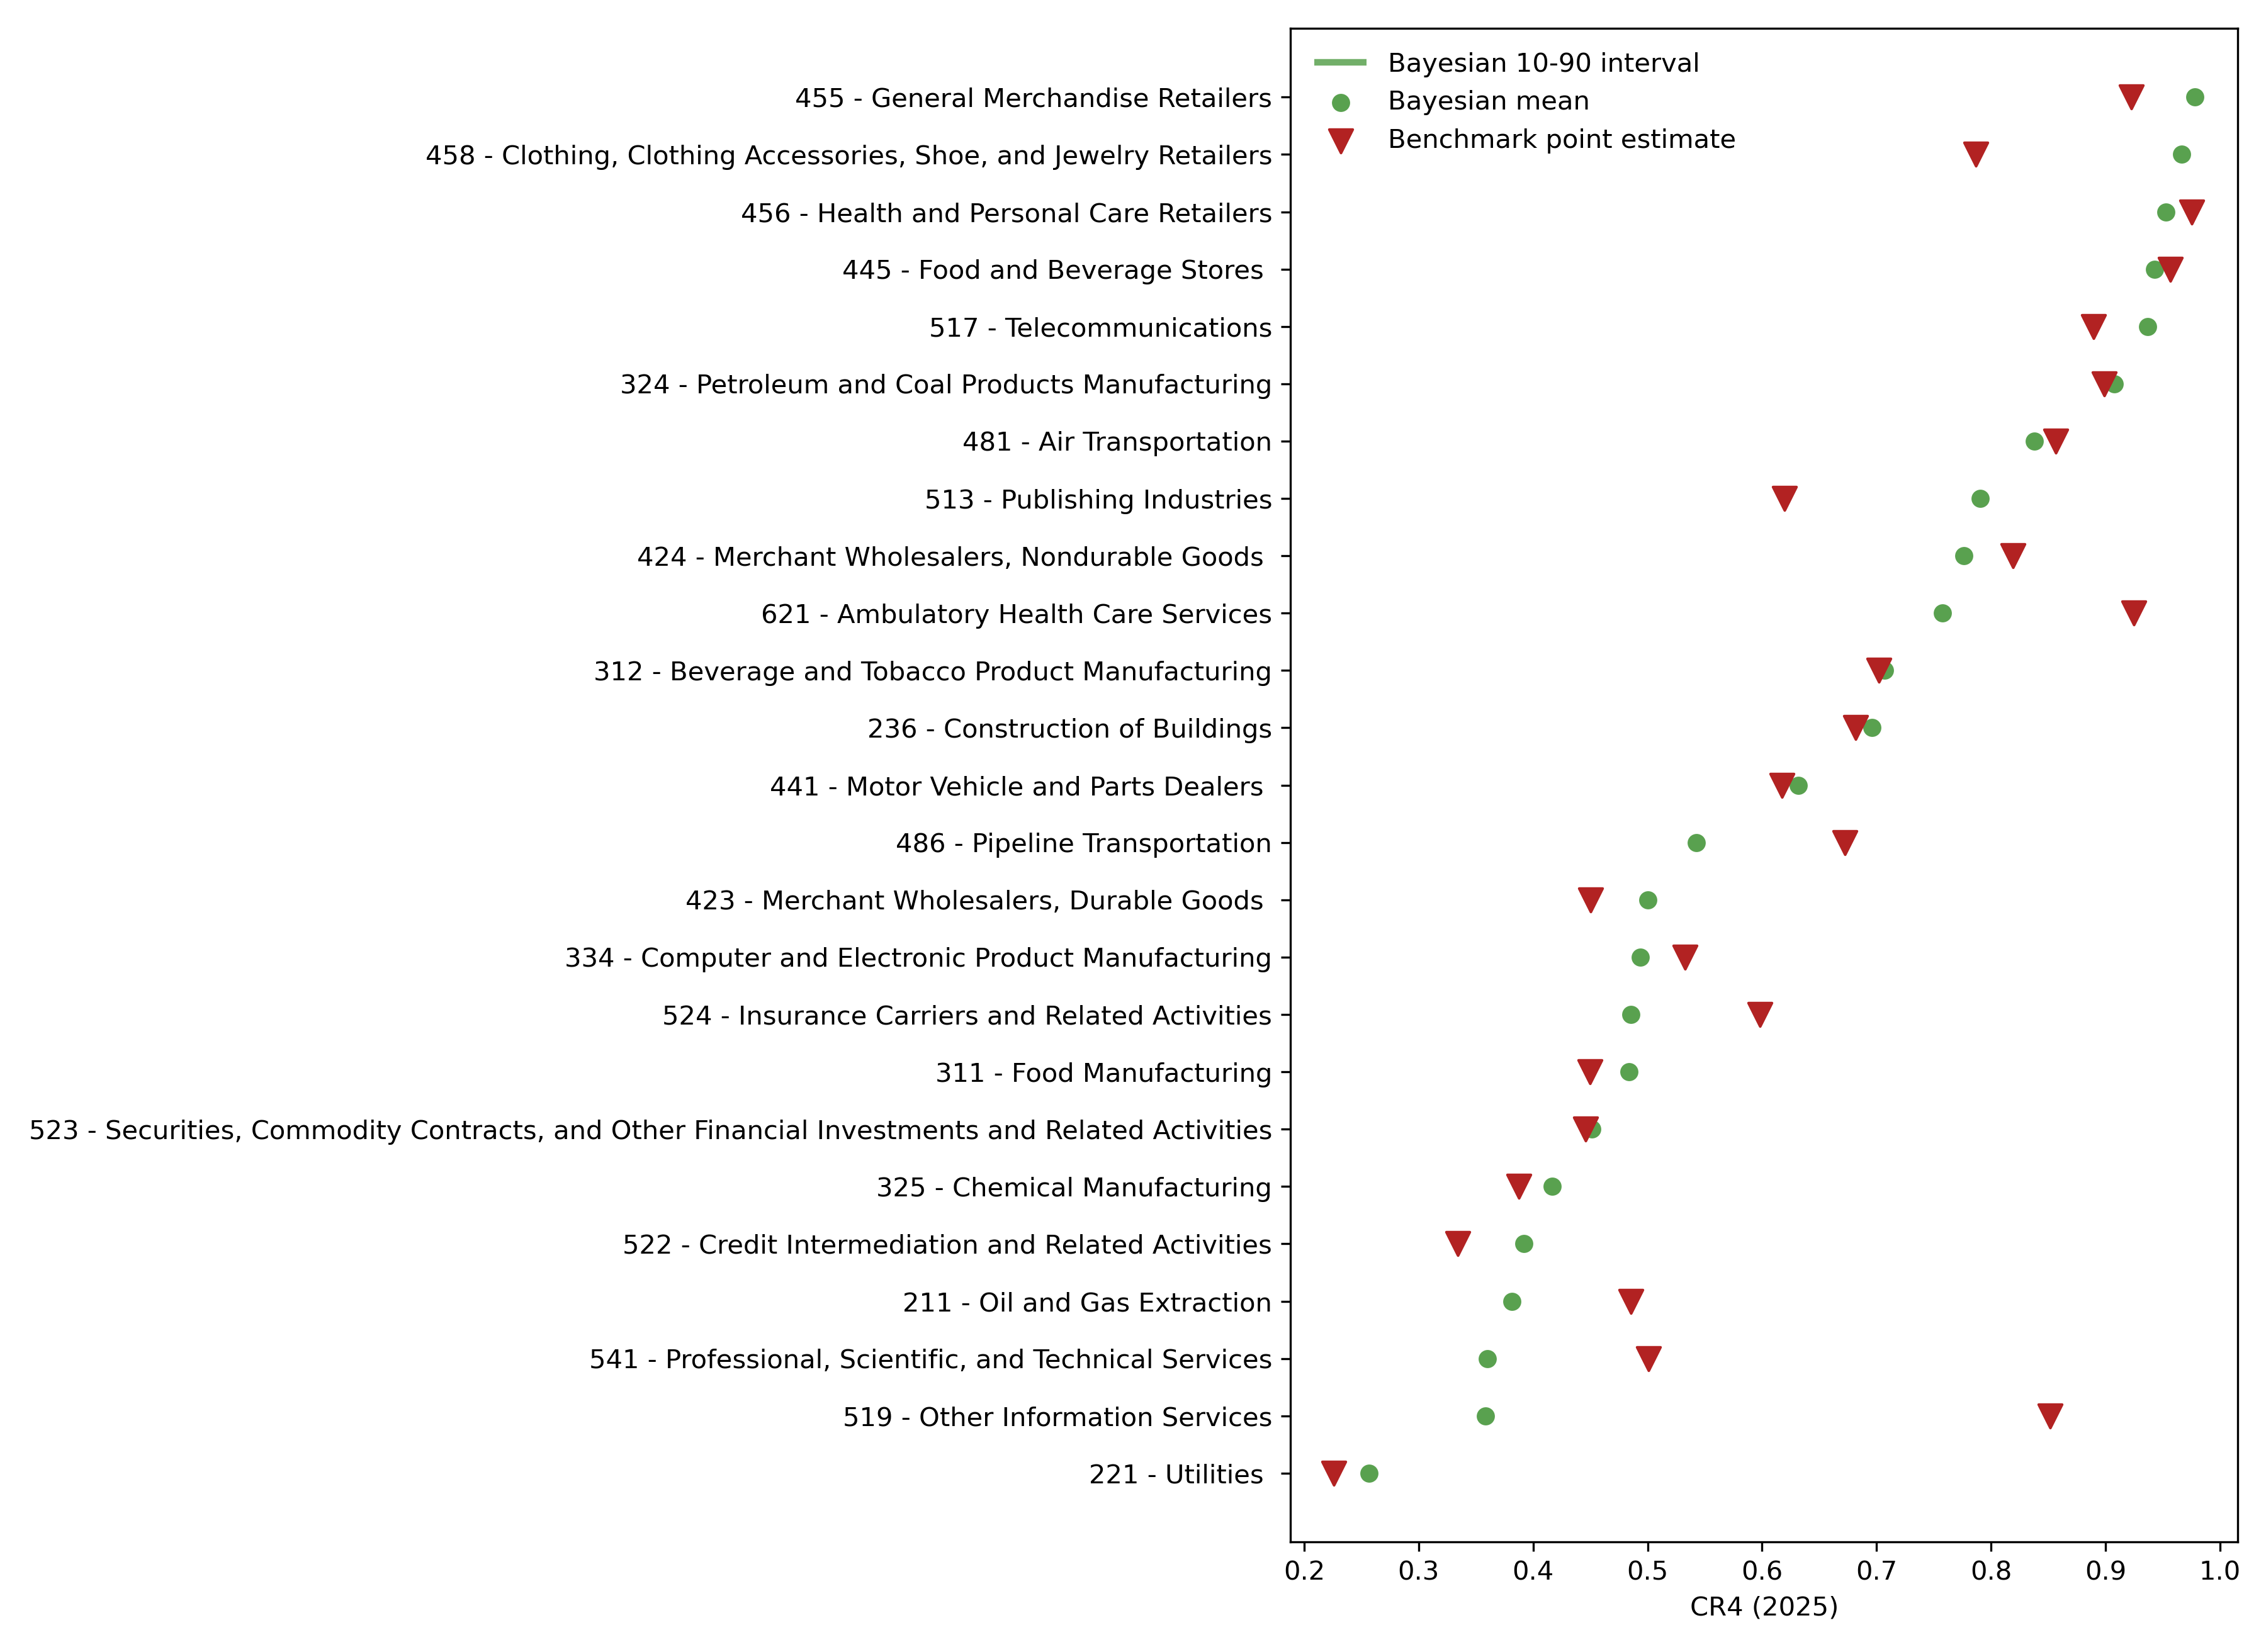
\includegraphics[width=0.5\textwidth]{../assets/figures/wrds/cr4_comparison_by_industry_2025.png}
  \end{center}

  \small Benchmark-posterior gap larger for CR4 than for HHI---fixed allocation inflates top-four share more aggressively than aggregate HHI.

\end{frame}

\begin{frame}[noframenumbering]{Appendix: Coverage by Year}

  % --- TABLE FONT SIZE: change \scriptsize below to \tiny or \footnotesize ---
  {\tiny              % <-- font size for this slide table
  \begin{tabular}{@{}lrrrrrr@{}}
\toprule
Statistic & \textbf{Firms} & \textbf{Current S\&P 500 firms} & \textbf{Segment-year observations} & \textbf{Segment-industry rows} & \textbf{Total sales} & \textbf{Total count mass} \\
\midrule
2017 & 1,728 & 168 & 1,797 & 3,698 & 3,930,581.97 & 5,397.00 \\
2018 & 2,037 & 197 & 2,139 & 4,472 & 5,739,931.17 & 11,463.00 \\
2019 & 2,238 & 205 & 2,365 & 4,990 & 6,565,124.91 & 18,042.00 \\
2020 & 2,228 & 207 & 2,347 & 5,457 & 6,436,082.00 & 18,312.00 \\
2021 & 2,228 & 207 & 2,355 & 5,636 & 7,196,233.59 & 18,171.00 \\
2022 & 2,209 & 206 & 2,329 & 5,119 & 7,954,570.72 & 17,943.00 \\
2023 & 2,148 & 207 & 2,261 & 4,795 & 8,248,851.77 & 16,542.00 \\
2024 & 2,024 & 203 & 2,102 & 4,365 & 8,260,132.23 & 10,818.00 \\
2025 & 1,508 & 197 & 1,571 & 3,240 & 8,116,667.43 & 4,821.00 \\
2026 & 34 & 11 & 36 & 72 & 1,267,646.34 & 108.00 \\
\midrule
All years & 2,932 & 241 & 19,302 & 41,844 & 63,715,822.11 & 121,617.00 \\
\bottomrule
\end{tabular}

  }
  \vspace{0.3em}
  %{\tiny\textit{Notes:} Firm counts = unique \texttt{gvkey}s in sales panel.
  %S\&P~500 flag is current membership (\texttt{curr\_sp500\_flag=1}).
  %Sales in millions USD. 2026 is partial (early filers only).}

\end{frame}

\begin{frame}[noframenumbering]{Appendix: Model Generalizes --- Amazon India (Kaggle)}

  \textbf{Same model, different data.}
  \begin{itemize}
    \item 1{,}465 Amazon India product listings; revenue $\propto$ price $\times$ rating count
    \item Brands $\leftrightarrow$ firm-segments \quad Categories $\leftrightarrow$ NAICS codes
    \item Keyword co-occurrence counts $\leftrightarrow$ NAICS linkage counts
    \item 20\% evidence sample with revealed categories updates posterior
  \end{itemize}

  \vspace{0.5em}

  \begin{columns}[T]
    \begin{column}{0.52\textwidth}
      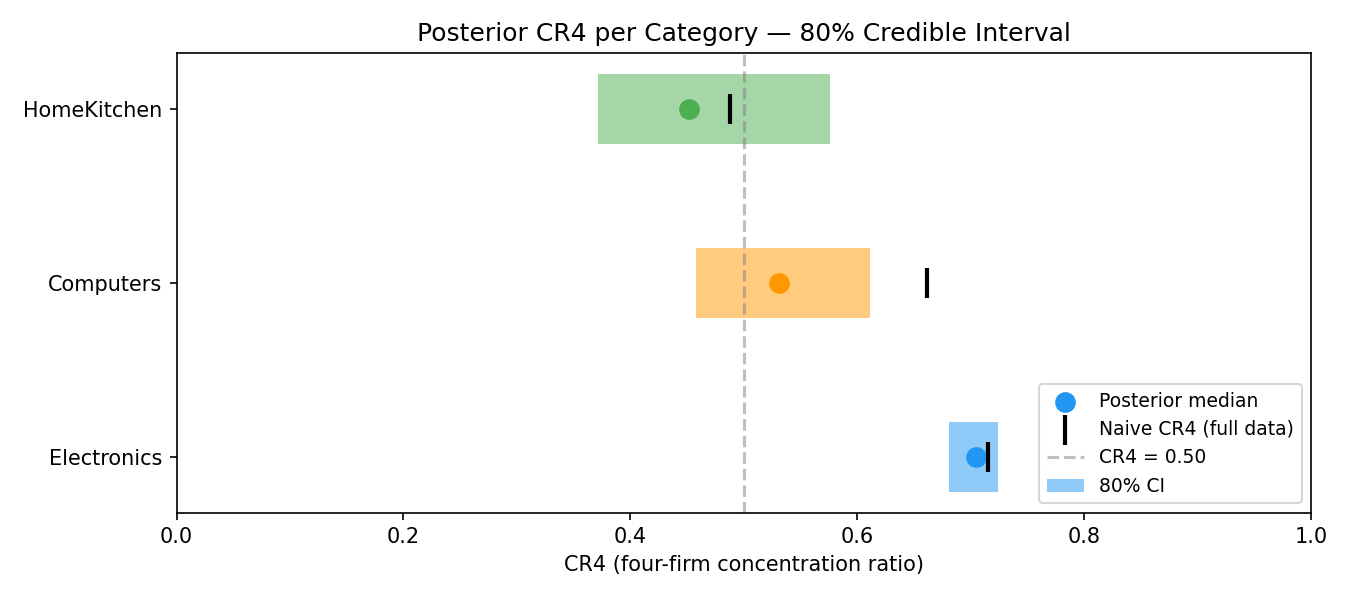
\includegraphics[width=\linewidth]{../assets/figures/demo/posterior_cr4_forest.png}
    \end{column}
    \begin{column}{0.46\textwidth}
      \vspace{0.5em}
      \textbf{Same pattern reappears:}\\[0.4em]
      Na\"{i}ve benchmark overstates CR4\\[0.3em]
      Largest gap in \textbf{Computers}:\\
      -- Bayesian: 0.53 [0.46, 0.61]\\
      -- Na\"{i}ve: 0.66 (outside CI)\\[0.3em]
      Electronics: near-agreement\\
      (allocation uncertainty is lower)
    \end{column}
  \end{columns}

\end{frame}

\end{document}
